\section{Sikkerhedsverifikation}
\begin{frame}{Sikkerhedsverifikation}{Omformulering af definition for barrierecertifikat}
	\vspace{3mm}
\begin{block}{SOSTOOLS}
	\begin{itemize}
		\item Metodisk måde at søge barrierecertifikat for et system og dermed sikkerhedsvalidere det
		\item Kræver omformulering til sum of squares (SOS) problem
	\end{itemize}
\begin{equation*}
p(\mathbf{x})=\sum\limits_{j=1}^{m}f_j^2(\mathbf{x})=\mathbf{z}^T\mathbf{Q}\mathbf{z}\quad \in\Sigma[\mathbf{x}]
\end{equation*}
\end{block}
	\vspace{-8mm}
\begin{minipage}[b]{0.57\linewidth}
	\phantom{.}
	\vspace*{6mm}
\begin{block}{Putinars Positivstellensatz}
	\begin{itemize}
		\item Gør det muligt at definere funktionens fortegn på de forskellige regioner
	\end{itemize}
	\vspace{5mm}
\end{block}
\end{minipage}
\hspace{1mm}
\begin{minipage}[b]{0.35\linewidth}
	\vspace{3mm}
	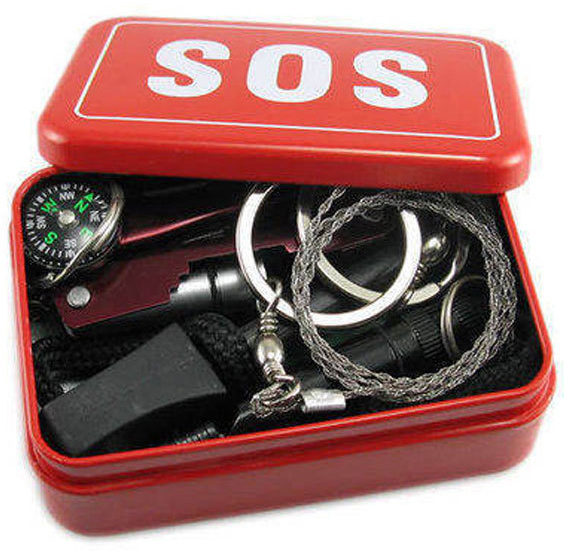
\includegraphics[width=1\textwidth]{sostools.jpg}
\end{minipage}
\end{frame}

\begin{frame}{Barrierecertifikat-søgning med SOSTOOLS}{Sikkerhedsverifikation af lukketsløjfesystem}
	\vspace{2mm}
\begin{minipage}[b]{0.35\linewidth}
	\begin{block}{Barrierecertifikat}
		\vspace{-5mm}
		\begin{align*}
		B(\mathbf{x})&\leq 0 \quad \forall\,\,\,\mathbf{x}\in\mathcal{X}_0\\
		B(\mathbf{x})&> 0 \quad \forall\,\,\,\mathbf{x}\in\mathcal{X}_u\\
		L_{f_{cl}}B(\mathbf{x})&\leq 0 \quad \forall\,\,\,\mathbf{x}\in\mathcal{X}
		\end{align*}
	\end{block}
\end{minipage}
\hspace{15mm}
\begin{minipage}[b]{0.4\linewidth}
%\begin{block}{Slide: beskrevet ved fejltilstand}
%	\begin{itemize}
%		\item 1.ordens-approksimering
%		\item 2.ordens-approksimering
%	\end{itemize}
%\end{block}
%\begin{figure}[h]
%\begin{subfigure}[h]{.3\textwidth}
%	\centering
%	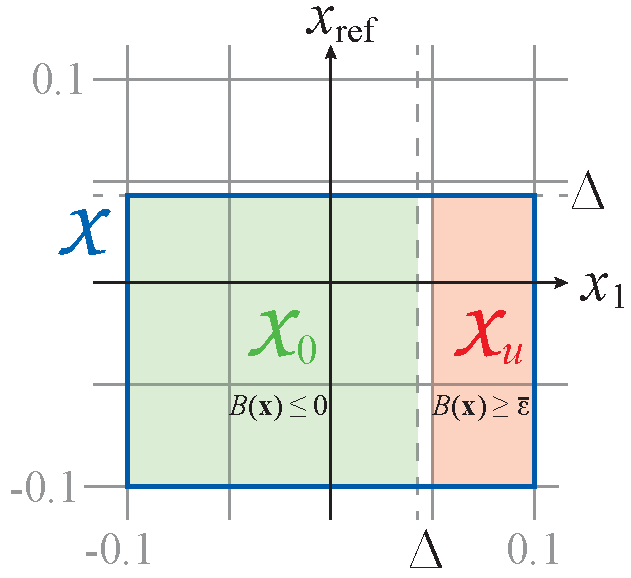
\includegraphics[width=0.3\textwidth]{sos_Xregion.pdf}
%\end{subfigure}
\hspace{3mm}
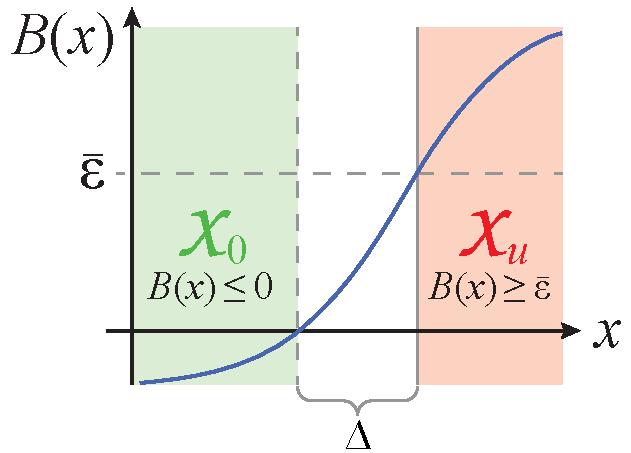
\includegraphics[width=\textwidth]{sos_delta.pdf}
%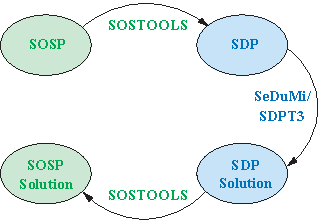
\includegraphics[width=1\textwidth]{SOSTOOLS.pdf}
%\begin{subfigure}[h]{.3\textwidth}
%	\centering
%	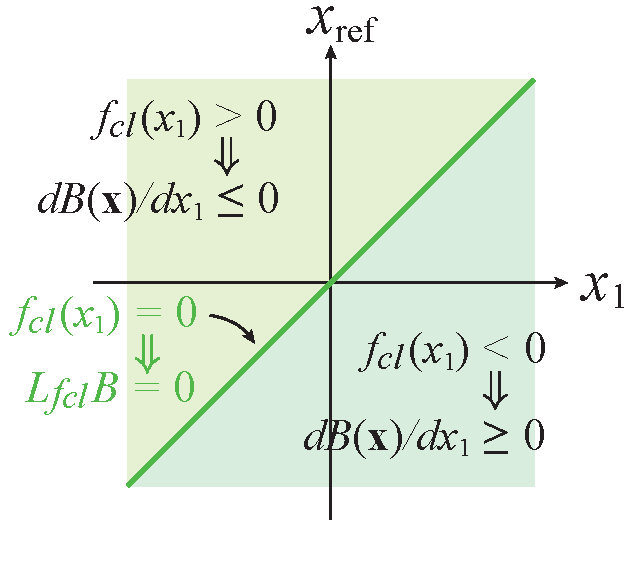
\includegraphics[width=0.4\textwidth]{sos_Xregion_dBdx.pdf}
%\end{subfigure}
%	\hspace{3mm}
%\begin{subfigure}[h]{.3\textwidth}
%	\centering
%	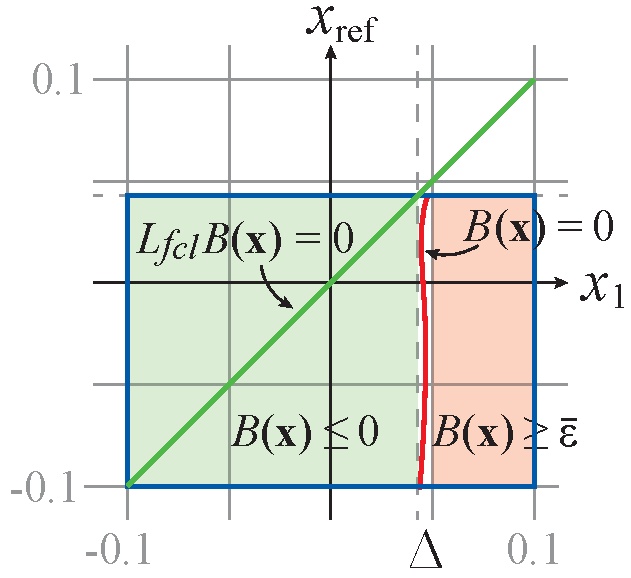
\includegraphics[width=0.3\textwidth]{sos_Xregion_Bvalue.pdf}
%\end{subfigure}
%\end{figure}
%\hspace{3mm}
%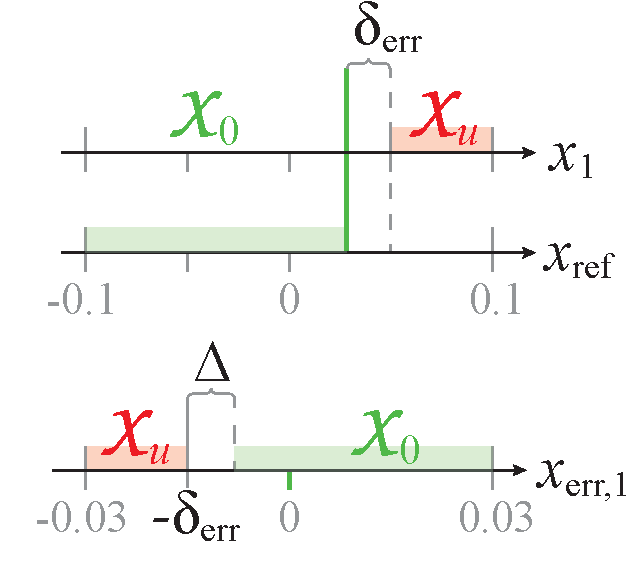
\includegraphics[width=0.4\textwidth]{sos_errorref_1d_new_2ndorder.pdf}
\end{minipage}

%\begin{minipage}[b]{0.65\linewidth}
\vspace{2mm}
%\begin{block}{Forståelse af værktøjet}
%		\begin{itemize}
%			\item Parametre til evaluering af resultat: feasibility ratio, residual norm, test om udtryk er SOS
%		\end{itemize}
%\end{block}
\begin{block}{Omformulering af barrierecertifikat}
	\vspace{-5mm}
	\begin{align*}
	&&	-B(\mathbf{x}) &\geq 0 \quad  \forall \hspace{2mm} \mathbf{x} \in \mathcal{X}_0 \quad \Leftarrow& 	-B(\mathbf{x}) - \sum q_jg_j &\,\,\,\in \Sigma[\mathbf{x}] &&& \\
	&&	B(\mathbf{x})-\bar{\epsilon} &\geq 0 \quad  \forall \hspace{2mm} \mathbf{x} \in \mathcal{X}_u \quad \Leftarrow& 	B(\mathbf{x})-\bar{\epsilon} - \sum q_jg_j &\,\,\,\in \Sigma[\mathbf{x}] &&& \\
	&&	-L_{f_{cl}}B(\mathbf{x}) &\geq 0 \quad  \forall \hspace{2mm} \mathbf{x} \in \mathcal{X} \quad\,\, \Leftarrow& 	-L_{f_{cl}}B(\mathbf{x}) - \sum q_jg_j &\,\,\,\in \Sigma[\mathbf{x}] &&& 
	\end{align*}
\end{block}
%\hspace{1mm}
%\begin{minipage}[b]{0.32\linewidth}
%\href{file:../../MATLAB/test_barriersearch.m}{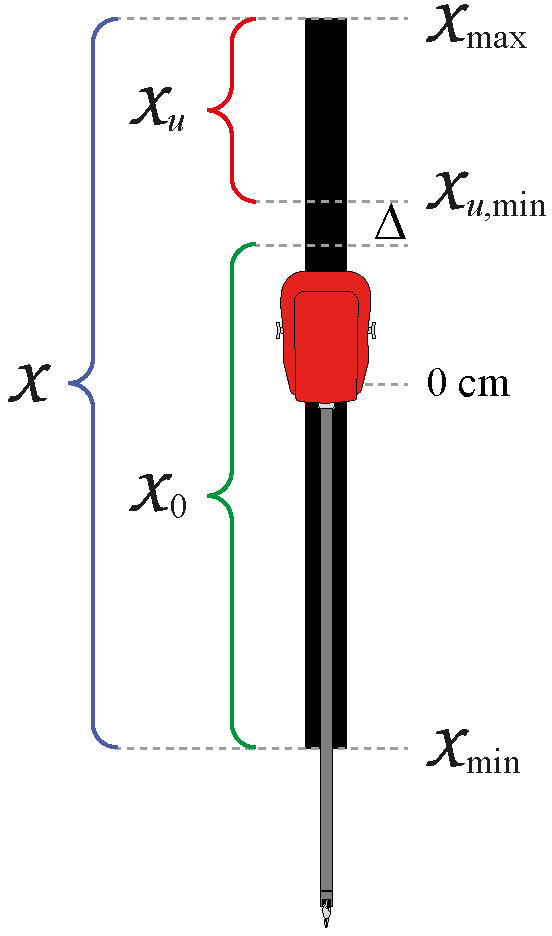
\includegraphics[width=1\textwidth]{slide_sos.pdf}}	
%\end{minipage}
\end{frame}

%\begin{frame}{Barrierecertifikat-søgning med SOSTOOLS}{Sikkerhedsverifikation gennem fejl-tilstand}
%	\begin{block}{Omformulering af problemet til fejl-tilstanden}
%		\begin{itemize}
%			\item Koordinatskifte og sammenhæng
%			\item Forsimpling af problemet -- sikkerhedsverificering af både første- og andenordens model af slide-bevægelse
%		\end{itemize}
%	\end{block}
%	\begin{figure}[h]
%%		\begin{subfigure}[h]{.3\textwidth}
%%			\centering
%			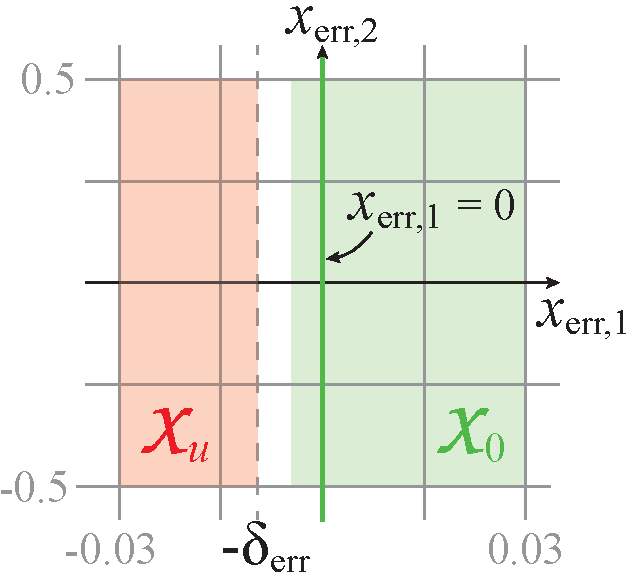
\includegraphics[width=0.3\textwidth]{sos_error_2d_2ndorder.pdf}
%%		\end{subfigure}
%		\hspace{3mm}
%%		\begin{subfigure}[h]{.3\textwidth}
%%			\centering
%			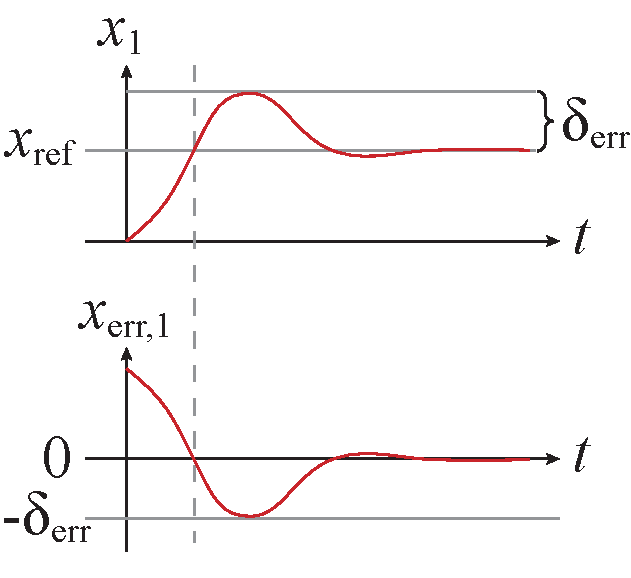
\includegraphics[width=0.3\textwidth]{sos_delta_error_2ndorder.pdf}
%%		\end{subfigure}
%		\hspace{3mm}
%%		\begin{subfigure}[h]{.3\textwidth}
%%			\centering
%			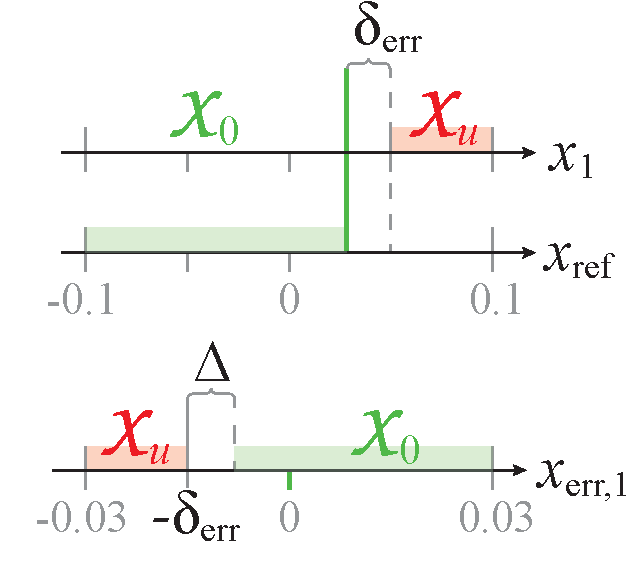
\includegraphics[width=0.3\textwidth]{sos_errorref_1d_new_2ndorder.pdf}
%%		\end{subfigure}
%	\end{figure}
%\end{frame}

%\begin{frame}{Evaluering af SOSTOOLS}{Sikkerhedsverifikation af lukketsløjfesystem}
%	\begin{block}{Evaluering af løsning}
%		\begin{itemize}
%			\item Feasibility ratio, residual norm, test om ligninger er SOS
%			\item Mange parametre at skrue på
%			\item Længere proces at minimere numeriske fejl
%		\end{itemize}
%	\end{block}
%	\begin{block}{Evaluering af værktøjet}
%		\begin{itemize}
%			\item Udviklet framework til søgning efter barrierecertifikater
%			\item Fundet mange brugbare løsninger
%			\item Systematisk afsøgning er en lang og iterativ proces
%			\item Avanceret metode der kommer til sin ret for højere-ordens systemer
%		\end{itemize}
%	\end{block}
%\end{frame}